% Basic US Letter document format
% by C. G. Wilson 

\documentclass[11pt]{article}
% \usepackage{palatino}
\usepackage{amsfonts}
\usepackage[pdftex]{graphicx}
\usepackage{caption}
\usepackage{subcaption}
\textwidth 6.85in
\textheight 8.75in

\pagestyle{headings}
\markright{\today, Whatever header}

\begin{document}
\oddsidemargin -0.22in
\evensidemargin -0.22in
\topmargin 0.05in
\topskip 0.25in
\headheight 0.05in
\headsep 0.25in





\begin{center}
\Large{\textbf{Results}}
\end{center}


\begin{figure}
	\centering
	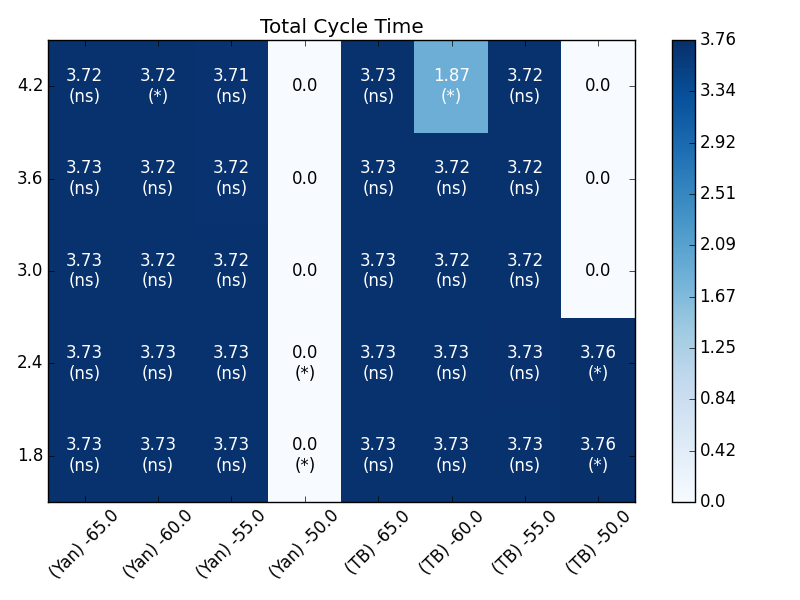
\includegraphics[scale=0.4]{heatmap_Total_Cycle_Time.png}
	\caption{Heat map showing variations in total cycle time with changes in $eL$, $g_{NaP}$, and model. Zeroes indicate tonic spiking.}
	\label{fig:hm_tct}
\end{figure}


\begin{figure}
	\centering
	\subcaptionbox{Time series for TB Model.\label{fig:ts_6042_tb}}
		{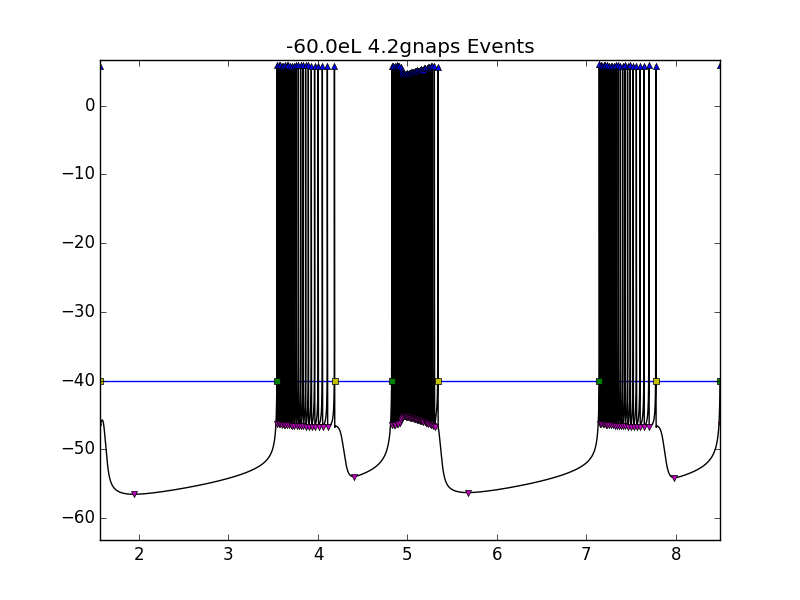
\includegraphics[scale=0.4]{time_ser_tb_-60p0eL_4p2gnaps.png}}%
	\subcaptionbox{Time series for Yan Model showing a single, consistent interburst interval width.\label{fig:ts_6042_yan}}
		{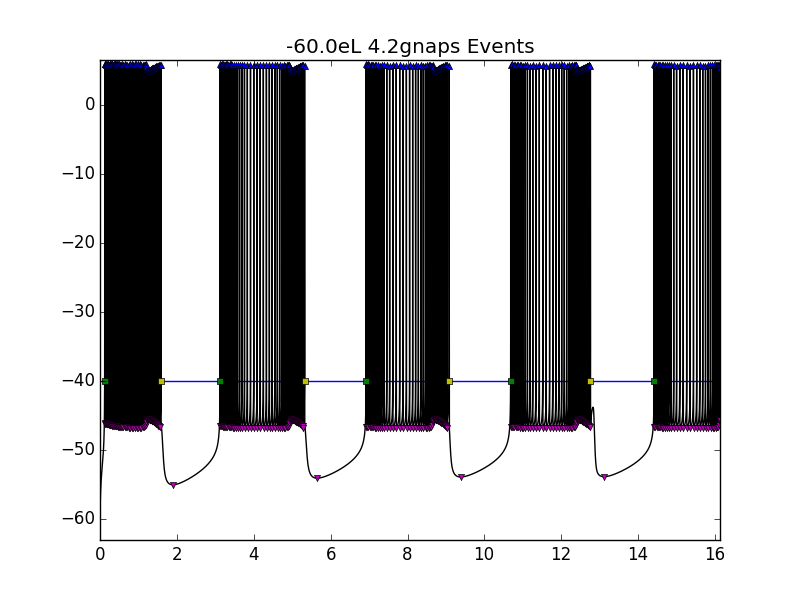
\includegraphics[scale=.4]{yan_-60p0eL_4p2gnapstime_series.png}}
	\caption{Time Series for Yan and TB models with $eL=-60 mV$ and $g_{NaP}=4.2 nS$. ~\ref{fig:ts_6042_yan} showing the two different interburst intervals.} \label{ts_6042}
\end{figure}

Average total cycle time, the time from the start of one burst to the start of another, was very uniform between models for all parameter sets that exhibited bursting (Fig [~\ref{fig:hm_tct}]). The only point of significant difference was at $eL=-60 g_{nap} = 4.2$ where the value for the TB model was half that of the Yan model, due to the two modes of interburst interval present in for the TB model but not for the Yan model (Fig [~\ref{fig:ts_6042}]).


   
\begin{figure}
\centering
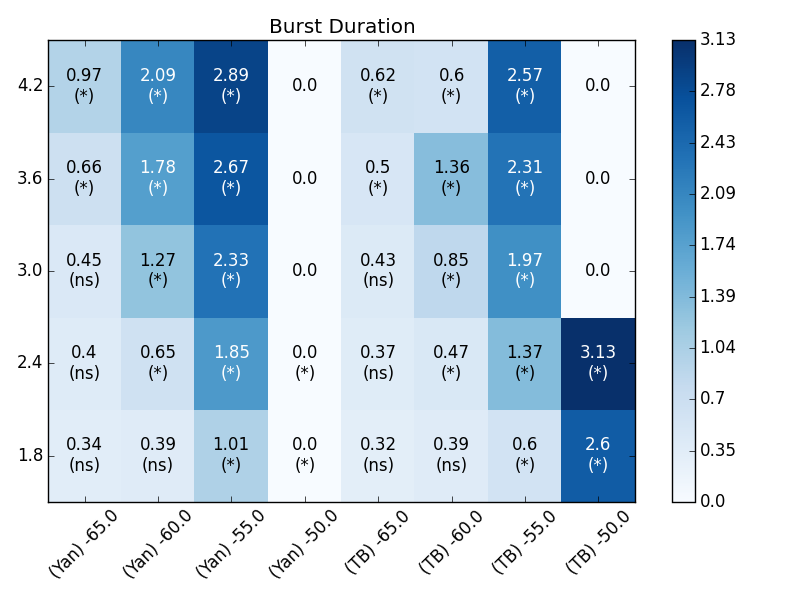
\includegraphics[scale=.4]{heatmap_Burst_Duration.png}
\end{figure}
Where bursting occurs in the Yan model, burst duration for Yan increases more rapidly than TB as $eL$ increases. For $eL=-55 mV$, burst duration is different at all tested $g_{NaP}$ values.
Differences in burst duration between the two models does not change significantly with change in $g_{NaP)$. For Yan, bursting does not occur while $eL = -50 mV$, while bursting occurs at $eL=-50,\  g_{NaP}=1.8, 2.4$. 

\begin{figure}
\begin{center}
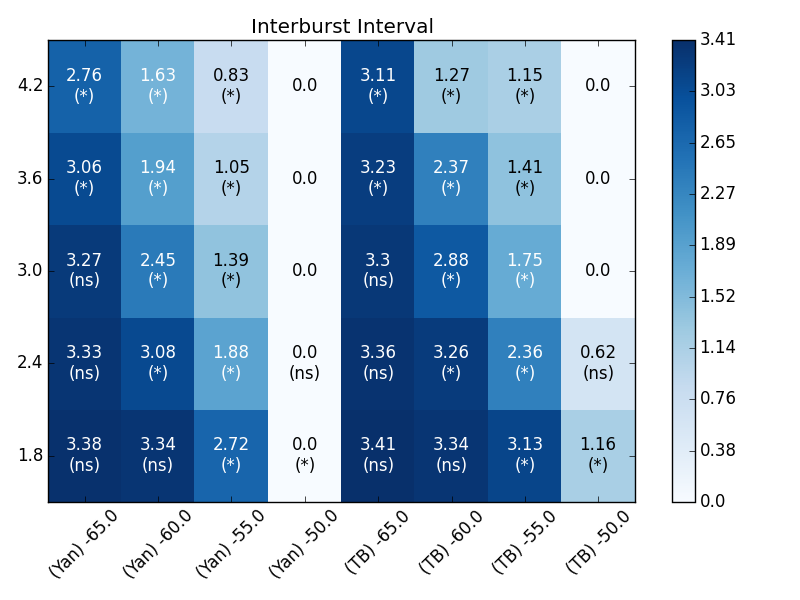
\includegraphics[scale=.4]{heatmap_Interburst_Interval.png}
\end{center}
\end{figure}

The same pattern that occurs in burst duration occurs in reverse for interburst interval. Since Total cycle time, the sum of burst duration and interburst interval, is largely static this is not surprising. The only exception, for $eL=-50.0,\ g_{NaP} = 2.4$ where interburst interval for the TB model shrinks to 0.62 seconds, which is apparently not significantly different from 0.
  
\begin{figure}
\begin{center}
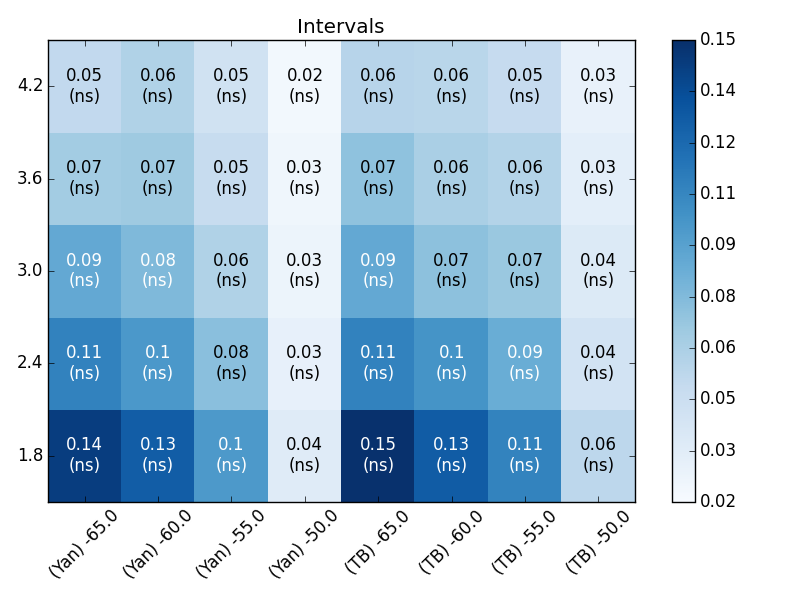
\includegraphics[scale=.4]{heatmap_Intervals.png}
\end{center}
\end{figure}
 
 
 \begin{figure}
\begin{center}
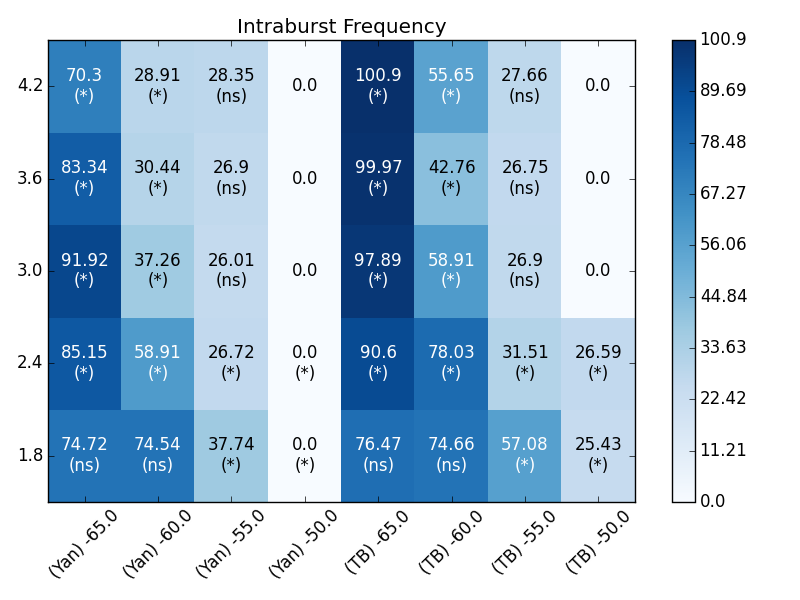
\includegraphics[scale=.4]{heatmap_Intraburst_Frequency.png}
\end{center}
\end{figure}
 
 \begin{figure}
\begin{center}
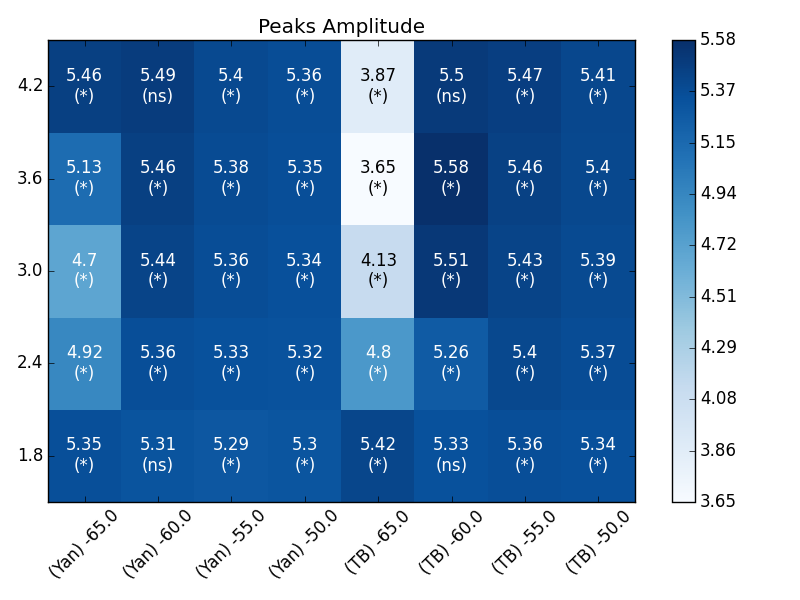
\includegraphics[scale=.4]{heatmap_Peaks_Amplitude.png}
\end{center}
\end{figure}
 
%\vspace{1.50cm}
%\noindent
\end{document}